\documentclass[11pt]{article}
\usepackage[T1]{fontenc}
\usepackage[utf8]{inputenc}
\usepackage{lmodern,amsmath,amssymb,graphicx,geometry,microtype,setspace,booktabs,caption}
\usepackage[hidelinks]{hyperref}
\geometry{letterpaper,margin=1in}
\setlength{\parindent}{0pt}
\setlength{\parskip}{0.55em}
\setlength{\emergencystretch}{2em}
\captionsetup{labelfont=bf,font=small}
\renewcommand{\refname}{References}
\pagestyle{empty}
\renewcommand{\thefigure}{S\arabic{figure}}
\setcounter{figure}{12}
\begin{document}
\begin{figure}[!ht]\centering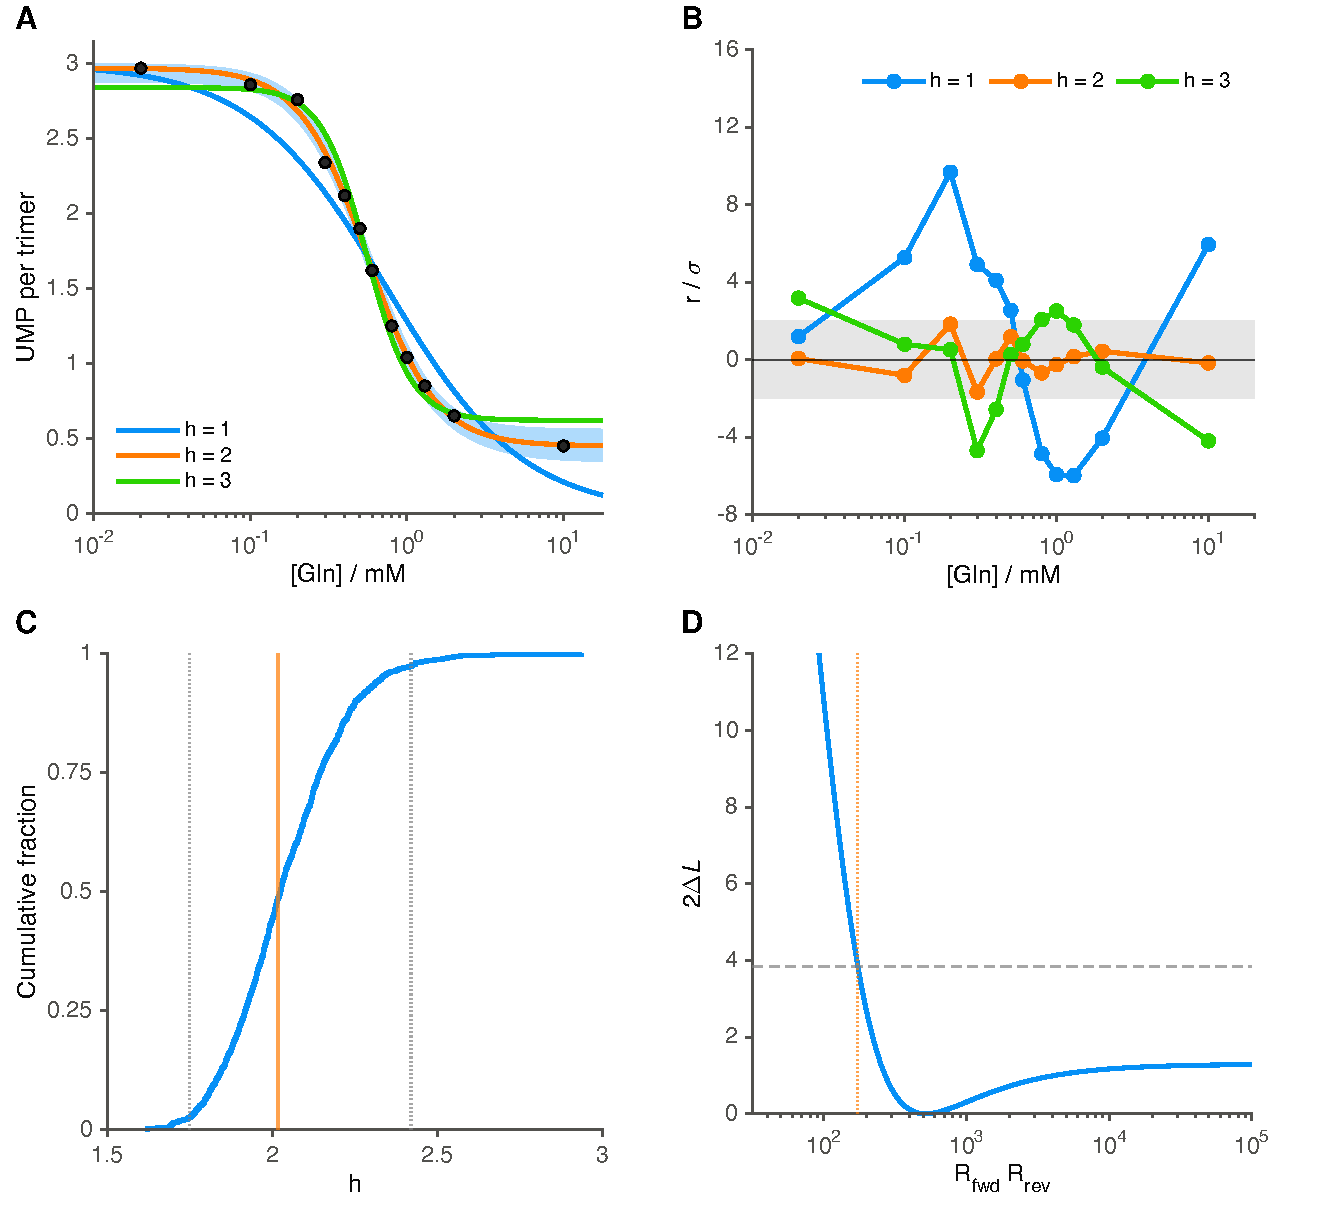
\includegraphics[width=\textwidth,height=0.60\textheight,keepaspectratio]{figure_inputs/FigS13_extended.pdf}\caption{\textbf{Information in the digitized first-layer titration.} (A) Digitized coordinates and bounded fits with h=1, 2, and 3. The fitted exponent, 2.018, nearly coincides with h=2. Shading spans pointwise 2.5th--97.5th percentiles under coordinate perturbations. (B) Fixed-exponent residuals divided by the common h=2 residual scale, approximately 0.0407 UMP per trimer. (C) Fitted-exponent cumulative distribution from 2,000 coordinate perturbations; dotted lines mark the central 95\% range. This is not an experimental replicate distribution. (D) Profile-likelihood loss for the regulatory swing. The horizontal criterion is 3.841 and its finite lower endpoint is approximately 173. The reciprocal-regulation interpretation is conditional on the plateau model.}


\end{figure}
\end{document}
